\chapter{Algoritm Implementation}
One of the first considerations when implementing a DSP algorithm in an embedded system is the choice of platform. 

We have worked with or been presented to several different platforms throughout the courses in our education. Those relevant here are the following:

\begin{itemize}
\item Blackfin
\item PSoC
\item DK8k
\end{itemize}

\begin{table} \label{tab:proscons}
    \begin{tabular}{l|ll}
    Platforms & Pros                          & Cons                           \\ \hline
    Blackfin  & FPU, fast, audio codec        & No prior experience            \\
    PSoC      & Well known                   & No FPU, slower, no audio codec \\
    DK8k      & Well known, fast, audio codec & No IDE                         \\
    \end{tabular}
\end{table}

To give a rough estimate of which platform would be the best suited for our project, table \ref{tab:proscons} gives a quick-and-dirty sketch of pros and cons for the various platforms. The purpose is not to decide based on those only, but to quickly see if any platforms can be ruled out early in the process.
We see that the best candidates for our system is DK8k and Blackfin. Because the DK8k has no IDE we would like to have a closer look at Blackfin. We have no prior experience with it - initially a con, but it can be an advantage to have the opportunity to work with a new platform as well and get to know it.
Based on that, we dive further into the specs of the Blackfin to see if it fulfills our requirements from the development phase and the system requirements.

\subsection{Blackfin}
\textbf{Speed:}\\
The blackfin processor runs at 600MHz. For every clock it can do two operations (multiplication and/or addition). This effectively means that we can do 1200 million operations per second, if we use the processor 100\% of the time.\\
\textbf{I/O:}\\
The blackfin has an output range of 0 - 0.4 V low to 2.4 - 3.6 high. Input range is -0.3 to 3.6 V. Most of the blackfins I/O is controlled by ports. All the phono plugs are connected to the port "Sport0". \\
\textbf{ADC \& Audiocodec:}\\
The blackfin has a built-in audiocodec consisting of 4 ADCs and 6 DACs with a resolution of 24 bits. It has a signal to noise ratio of 105dB\footnote{http://www.analog.com/en/audiovideo-products/audio-codecs/ad1836/products/product.html}. There is an example project in the VisualDSP++ environment explaining how to utilize this codec.\\
\textbf{Memory:}\\
The blackfin got a 32Kb L1 Data SRAM (see figure \ref{img:mem_table}). Using the 16-bit data type "short", there is memory enough for a 16K samples, which - according to our algorithm development - should be sufficient for cross-correlation.
\begin{figure}[hbpt]
\centering
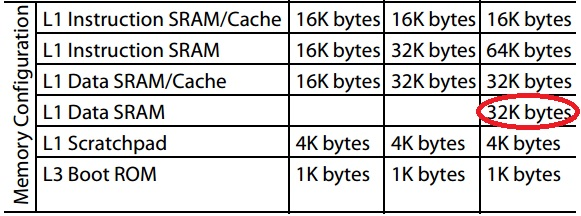
\includegraphics[width=0.5\textwidth]{billeder/memorytable}
\caption[Screen dump from datasheet]{Screen dump from datasheet\footnotemark}
\label{img:mem_table}
\end{figure}
\footnotetext{\url{http://www.analog.com/static/imported-files/data_sheets/ADSP-BF531_BF532_BF533.pdf}}

Overall the blackfin fulfills our requirements to the platform. 
When working with embedded signal processing, one of the ever occurring decisions to be made is whether to use floating og fixed point data format. 

\section{Fixed-/Floating Point}
\subsection{Floating Point}
Floating point is a way of give approximation of a real value. Usually when working with floating point we have a fixed number of significant digits. A way of presenting a floating point number is "1.2345". Floating point types in c are double and float. The main advantage of floating point is high precision. This comes at a cost of performance and component price. Some embedded microprocessors can not process floating point as it requires a floating point unit(FPU).\\
\subsection{Fixed Point}
Fixed point arithmetic is a way to represent a number that has a fixed number of digits before and after the the decimal "." point. Fixed point arithmetic is especially useful for representing fract data types in base 2 or base 10. A way to represent "1.23" in fixed point is "1230". A scaling factor is used. Scaling factors are usually base 2 or base 10. The main advantage of fixed point is performance. This comes at a price of precision.\\
\subsection{Choice}
So as always we have to choose between performance and price on one hand and precision on the other. To make a better decision, we looked at performance using the different data types. In table \ref{tab:performance}, we look at 32-bit c integers, 32-bit assembly integers, float and 16-bit assembly integers (short). It is very clear that there are a huge performance loss (factor 5) in working with float compared to fixed point. This is as we would expect. Also we see that there is a factor 6 performance loss using c-style integers instead of assembly integers. This is a valuable observation when optimizing our system later on.
Because of our real-time demand we need the processing power saved by using fixed point annotation instead of floating point. Assembly not being part of the scope for this course we chose for our first iteration to implement our application in c instead of assembly due to way better experience with c.

\begin{table}[hbtp]
	\centering
    \begin{tabular}{| p{4.5cm} | p{2.5cm} |}
    \hline
    Format                   & Clock cycles \\ \hline
    C style integer, 32 bit  & around 3000  \\ \hline
    Assembly integer, 32 bit & around 500   \\ \hline
    Float                    & around 16000 \\ \hline
    Assembly short, 16 bit   & around 70    \\ \hline
    \end{tabular}
    \caption{example of multiplication performance table}
    \label{tab:performance}
\end{table}

We have chosen the platform, the language and data type. Next is setup of the blackfin, were we have to consider several areas.

\subsection{Memory}
The blackfin has 2 types of memory: Internal and external. The internal SRAM consist of fast memory that is close to the processor.  As previously mentioned the L1 Data SRAM size is 32K Bytes. If we were to chose large arrays for our sound array we could enable the external SDRAM as well. This would provide us with a grand total of 132M bytes of memory. The SRAM is based on Harvard Architecture which makes it as fast as the processor. The SDRAM runs slower than the SRAM, so it would be ideal to confine the project to SRAM only. Enabling the SDRAM is done in VisualDSP++ by entering Project Options. The path would then be:
\begin{verbatim}
Project -> Link -> Processor (1) -> Memory Usage
\end{verbatim}

\subsection{DMA}
The DMA is a controller circuit on embedded units that can initiate memory read or write cycles. Before the DMA controller can be used we have to initiate it. The DMA controller on the blackfin can move data between L1 Cache, Flash or SDRAM and units connected to the DMA Access Bus. The scope of our project means that we have to use Sport0 (which will be connected to the audio connectors) and internal memory from the L1. \\

\subsubsection{Setup}
The DMA is setup using SPI on the blackfin. We have used code from the example project "Audio Talk-Through" Which initiates the dma channels 1, 2 and 5 for input, output and moving data to the built in audio codec. The DMA has the following init parts:
\begin{lstlisting}[language=C]
*pDMA1_PERIPHERAL_MAP // What to map the DMA to.
*pDMA1_CONFIG // which configuration your want.
*pDMA1_START_ADDR // Start address of the buffer.
*pDMA1_X_COUNT // Number of transfers
*pDMA1_X_MODIFY // Number of bytes between each transfer
\end{lstlisting}
In our setup we are using 32 bytes so the DMA in- and output are set to 32 bytes, 8 bursts of 4 bytes at a time. We map the in and output dma channels to Sport0 Rx and Tx. Sport0 is connected to our physical ports described below. The last thing we have to do is enable the DMA channels and that is done with the \begin{quote}
"DMAEN" flag in the "pDMA1\_CONFIG".
\end{quote}

\subsection{Buffer sizes}
We started by using 24000 size arrays. This means we had to use SDRAM. In an attempt to squeeze more performance out of our system we tried to limit ourselves to SRAM. The largest possible c style short array would be around 16000 elements. The next step was to try cross correlation with 2 16000 element signals. The cross correlation looked strange and somehow some of the cross correlation array was assigned to "unassigned" memory space.\\
The next step in the choice of buffer size was to look at the arrays we made in matlab. We asked ourselves what the smallest possible array with chirp and noise we could play with 48kHz was. We tried playing a 1000 sample chirp and found that it didn't play properly. The next step was to double the size to 2000. This time the chirp played properly.\\


\section{Blackfin Setup}
\subsection{DMA}

\subsection{Sport0}
The Sport0 is set up using the table \ref{table:Sport0}
\begin{table}[htbp]
    \begin{tabular}{| p{1.5cm} | l | p{4.5cm} | p{4.5cm} |}
    \hline
    C++ def      & Comment                   & Clear bit to 0                                   & Set bit to 1                             \\ \hline
    TFSR RFSR   & Frame sync required 		 & Does not require frame sync for every word & Requires frame  					sync for every word \\ \hline
    ITFS IRFS   & Internal frame  					sync & Use external  					frame sync                    & Use internal  					frame sync            \\ \hline
    ITCLK IRCLK & Internal clock            & Use external  					clock                         & Use internal  					clock                 \\ \hline
    TSPEN RSPEN & Enable                    & Disable transmit  					or receive                & Enable transmit  					or receive         \\ \hline
    \end{tabular}
    \caption{Sport0 Initialization}
    \label{table:Sport0}
\end{table}
Our Sport0 is set up the same way as the "talkthrough" project with: "External CLK, External Frame sync, MSB first". MSB first is instantiated by writing SLEN$\_$32 to the second register. Lastly we enable it by writing "TSPEN" and "RSPEN" to the registers pSPORT0 TCR1 and RCR1.
\subsection{Interrupts}
Interrups are set up using the 4 registers SIC$\_$IAR0 to 2 and SIC$\_$IMASK. We want to use DMA1 (Sport0 RX) Interrupt so we set the second word of the SIC$\_$IAR1 to 2. We also have to register ISR handlers to Sport0 and then enable interrupt. The interrupt code will then be:
\begin{lstlisting}[language=C]
*pSIC_IAR0 = 0xffffffff;
*pSIC_IAR1 = 0xffffff2f; // DMA1 (Sport0 RX)
*pSIC_IAR2 = 0xffffffff;

register_handler(ik_ivg9, Sport0_RX_ISR); //Handler

*pSIC_IMASK = 0x00000200; // enable interrupt
\end{lstlisting}




\subsection{Output}
\textbf{Sound}:\\
The original scope of our project was to have an audio source as our output, while using a sound to measure distance. This worked well since we already had the knowledge from the talkthrough on how to output sound.\\
We have a multitude of ways to create the sound we are playing. We could either create a sound in matlab and load it or we could create it directly on the blackfin. For testing purposes we chose the matlab solution. This would mean that once we have made the soundbits we wanted to use, we would have to convert them to a format known by the blackfin.





\subsection{Resources}
Regarding resources on the blackfin we are looking to try to make our own implementation through the project and then compare with the built-in function. We are not trying to do it better but rather get the understanding of what is going on.
We also want to investigate the use of DMA on the blackfin so we do not waste resources on moving data only processing it.



\subsection{Built-in functions}
\begin{lstlisting}[language=C]
short sin_fr32(short x);\\
\end{lstlisting}
The built-in sin function takes in a value x, which represents time or to be more exact the length on the x-axis. So for example for x=3.1415 the output will be ~0. It returns the value on the y axis. To use the function properly you need to calculate the value in each quandrant of the unit circle. In the documentation in VisualDSP++ it is described how to calculate this. We decided not to use this function since we figured a lot of math was involved which would slow our system.

\begin{lstlisting}[language=C]
void crosscorr_fr32 (	const short    samples_x[ ], 
                     	const short    samples_y[ ],
                     	int            sample_length,
                     	int            lags,
                     	short          correlation[ ]);
\end{lstlisting}
The built-in cross correlation function takes in the two signals, in our case the output array, and the recorded array. Sample\_length is the length of the input arrays, and lags is the number of elements in the array for the cross correlation, correlation[].\\
The function is extremely easy to get going with and very simple to use. Although it can take a long time to process large arrays, so it doesn't scale very well.\\
\subsection{Output}
\textbf{Sound and Decimation}:\\
The output sound is generated via. decimation and the fact that the system constantly outputs samples with 48kHz.\\
In matlab we generated a signal of one period with 2000 samples. Running through this one at a time once every 1/48kHz would make an output frequency of: $\frac{48000Hz}{2000}=24Hz$. This is a very low frequent sound so we needed to step faster through this period. A step of 30 each time would give an output frequency of $\frac{48000Hz}{\frac{2000}{30}}=720Hz$. We figured this was nice for a distance of 0mm. Our calculation of distance returnes the distance in mm and since we measure around 3m it would be way to large, since a step of 3030 would go more then through the array with the period making some aliasing problems. We choose to convert the distance from mm til decimeters. This means we go from steps of 30 to steps of 60, making the highest frequency $\frac{48000Hz}{\frac{2000}{30}}=1440Hz$. The frequencies are very distinguishable and also pleasant to hear.\\
\textbf{UART}\\
\subsection{Output frequency}

\subsection{Convert to BF}
The blackfin has a small "hack" when it comes to loading sound from memory:
\begin{lstlisting}[language=C]
short sound_buffer[length_of_signal] = { 
#include "signal_you_want_to_use.hex"
};
\end{lstlisting}
This means we have to convert our sound array to a hex format. The first thing we do when converting is reducing the amplitude of the signal to make sure it fits in a "c style short" datatype. Then we use a function "mydec2hex" which is an improved version of matlabs built-in function "dec2hex". After converting to hex-format we use the file descriptor to save the data into a hex file. The hex file is put in the project folder in VisualDSP++ and the codehack is put where you initialize your variables.



\subsection{IDE: VisualDSP++}
\subsubsection{Plot}
VisualDSP++ has a built-in function to plot data from the memory of the blackfin. This feature can be used when the blackfin has been flashed and then subsequently halted. To access this feature go into:
\begin{verbatim}
View -> Debug Windows -> Plot -> New
\end{verbatim}
Set name, length and type of the data you want to plot and press \"Add\". This way you can have multiple plots on the same graph. It is also possible to have multiple plots and to save the setting of your plot. An example of plot can be seen on figure~\ref{fig:visualdspplot}.
\begin{figure}[hbpt]
\centering
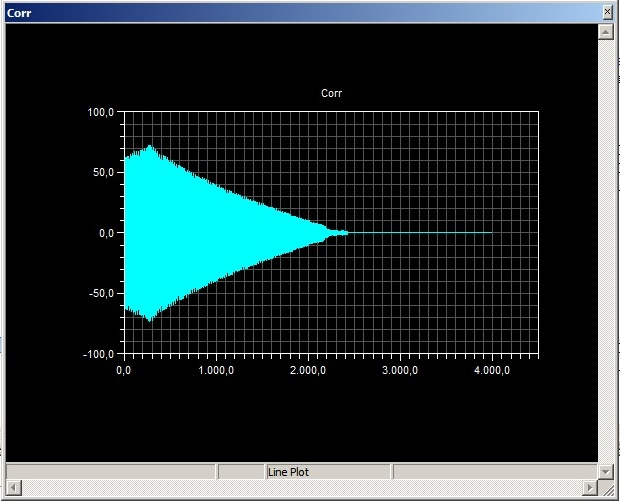
\includegraphics[scale=0.5]{billeder/visualdspplot}
\caption{Plot in VisualDSP++}
\label{fig:visualdspplot}
\end{figure}
\subsubsection{Memory dump}
A useful feature in VisualDSP++ is Memory dump. We can save the contents of arrays and variables directly onto the computer running VisualDSP++ in ".dat" format. To access this feature go into:
\begin{verbatim}
Memory -> Dump
\end{verbatim}
Set filename, type, size and variable/array name. Matlab can import these files directly.



\section{System overview/architecture}
hest

\section{Code functions}
\textbf{Defines:}\\

\subsection{Process\_data}
\subsubsection{Responsibility}
The responsibility of this c-file is to handle the data. It consist of two functions described below.
\subsubsection{Function descriptions}
\begin{table}[H]
\begin{tabular}{l p{12.5cm}}
\multicolumn{2}{l}{\texttt{\textcolor{blue}{void} Process\_Data( \textcolor{blue}{void})}} \\
\hline
Description:& The function handles input and output data, both chirp output and the sound for distance output. Depending of flags it records and plays audio.\\
Parameter(s):&None\\
Return:&None\\
\end{tabular}
\end{table}
\begin{table}[H]
\begin{tabular}{l p{12.5cm}}
\multicolumn{2}{l}{\texttt{\textcolor{blue}{int} totaldist calc\_dist( \textcolor{blue}{short*} corr)}} \\
\hline
Description:& The function calculates the distance to the object using the correlation array "corr".\\
Parameter(s):&\texttt{\textcolor{blue}short*} corr\\
Return:&\texttt{\textcolor{blue}int} totaldist\\
\end{tabular}
\end{table}

\textbf{calc$\_$dist}:\\
\begin{lstlisting}[language=C]
int time = 0;
int fs = 48;
int velocity = 340;
int dist = 0;
int totaldist = 0;
int numDist = 0;
int sound_factor=0;
int avg = 10;
int place = 0;
int myCount = 0;
int maxNum = 0;
int olddist = 0;
//filter coeficients:
float alpha = 0.3;

int calc_dist(short* corr){
	maxNum = 0;
            
	for(myCount = 0; myCount < SAMPLES; myCount++)
	{
		if(corr[myCount] > maxNum)
		{
			maxNum = corr[myCount];
			place = myCount;	
		}
		if(myCount == (SAMPLES - 1))
		{
			time = (place*100)/fs;
			dist = (1.096*(time * velocity)/200)-425;
		}
	}
	//average distance:
	olddist = totaldist;
	totaldist = dist*alpha + olddist*(1-alpha);
	
	sound_factor = totaldist/100;
	return totaldist;	
}
\end{lstlisting}
\textbf{Discription of calc$\_$dist function:}\\

\textbf{Process$\_$Data}:\\
\begin{lstlisting}[language=C]
void Process_Data(void)
{
	// Output Del
	if(num1>OUTPUTLEN){
		playFlag = 0;
	}
	if(playFlag){
		yn = (sound[num1] << 2);
		iChannel0LeftOut = (yn << 16);
			
	}
	
	if(num1>INPUTLEN){
		recFlag = 0;
	}
	if(recFlag)
	{
		soundIn[num1] = (short)(iChannel0LeftIn >> 14);
	}
	num1++;
	num2 = num2 + 20 + sound_factor; //Soundfactor is the distance in 1/10 meter
	num2 = num2 % 2000; 	// because the sinus buffer is 2000 samples
				// we want the remainder of 2000
				//because maybe num2 become more 
				//then just 1 more the 2000 
				//and we want the sinus to flow
	
	if(num1>5000){
		doX = 1;
	}
	xn = sinus[num2];
	
	iChannel0RightOut = (xn << 16);
}
\end{lstlisting}

\section{Signal/datatypes}
\section{Our Xcorr}
Description\\
Implementation\\